% Rapport de Stage -- ESIR
% Alexandre RIO
% merci à Florent GUIOTTE pour le template de base
\documentclass[a4paper,12pt,twoside,final]{article}

\usepackage[english,french]{babel}
\usepackage[utf8]{inputenc}
\usepackage[T1]{fontenc}
\usepackage[pdftex]{graphicx}
\usepackage{setspace}
\usepackage{hyperref}
%\usepackage[french]{varioref}
\usepackage{fancyhdr}
\usepackage{lmodern}
\usepackage[numbers,comma]{natbib}
\usepackage{xcolor}
\usepackage{titlesec}
\usepackage{listings}
\usepackage{graphicx}
\usepackage{pdfpages}
%\usepackage{wrapfig}
\usepackage{numprint}
\usepackage{listings}
\usepackage{pdflscape}

\lstset{tabsize=4,
        basicstyle=\scriptsize,
        %upquote=true,
        aboveskip={1.5\baselineskip},
        columns=fixed,
        showstringspaces=false,
        extendedchars=true,
        breaklines=true,
        prebreak = \raisebox{0ex}[0ex][0ex]{\ensuremath{\hookleftarrow}},
	frame=single,
        showtabs=false,
        showspaces=false,
        showstringspaces=false,
        identifierstyle=\ttfamily,
        keywordstyle=\color[rgb]{0,0,1},
        commentstyle=\color[rgb]{0.133,0.545,0.133},
        stringstyle=\color[rgb]{0.627,0.126,0.941},
	language=Java
}

\lstnewenvironment{java}[1][]{\lstset{tabsize=4,
        basicstyle=\scriptsize,
        %upquote=true,
        aboveskip={1.5\baselineskip},
        columns=fixed,
        showstringspaces=false,
        extendedchars=true,
        breaklines=true,
        prebreak = \raisebox{0ex}[0ex][0ex]{\ensuremath{\hookleftarrow}},
	frame=single,
        showtabs=false,
        showspaces=false,
        showstringspaces=false,
        identifierstyle=\ttfamily,
        keywordstyle=\color[rgb]{0,0,1},
        commentstyle=\color[rgb]{0.133,0.545,0.133},
        stringstyle=\color[rgb]{0.627,0.126,0.941},
	language=Java,
	label={#1},caption={#1},%avec nom du listing}
}}{}

\lstnewenvironment{javan}[1][]{\linespread{1}\lstset{	
	numbers=left,
	tabsize=4,
        basicstyle=\scriptsize,
        %upquote=true,
        aboveskip={1.5\baselineskip},
        columns=fixed,
        showstringspaces=false,
        extendedchars=true,
        breaklines=true,
        prebreak = \raisebox{0ex}[0ex][0ex]{\ensuremath{\hookleftarrow}},
	frame=single,
        showtabs=false,
        showspaces=false,
        showstringspaces=false,
        identifierstyle=\ttfamily,
        keywordstyle=\color[rgb]{0.1,0.1,1},
        commentstyle=\color[rgb]{0.133,0.545,0.133},
        stringstyle=\color[rgb]{0.627,0.126,0.941},
	language=Java,}
}{}

\colorlet{maincolor}{blue!30!black!79!white}
\colorlet{glocolor}{blue!50!white}
\colorlet{subgray}{white!20!black}
\colorlet{subsubgray}{white!40!black}

% Repport
\newcommand{\reporttitle}{Développement d'un générateur de code pour le développement basé sur le paradigme du model@runtime}     % Titre
\newcommand{\reportsubject}{Rapport de stage \\\large École supérieure d'ingénieurs de Rennes} % Sujet
\newcommand{\reportauthor}{Alexandre \textsc{Rio}} % Auteur
\newcommand{\reporteta}{esir}

% University
\newcommand{\univname}{\textsc{Esir}} % Name
\newcommand{\univaddra}{Université de Rennes 1} % Address line 1
\newcommand{\univaddrb}{Campus de Beaulieu \\ \numprint{35042} \textsc{Rennes} Cedex} % Address line 2
\newcommand{\univlogo}{images/logo_esir.pdf} % Logo

% Company
\newcommand{\compname}{\textsc{IRISA Rennes}} % Name
\newcommand{\compaddra}{Campus de Beaulieu} % Address line 1
\newcommand{\compaddrb}{263 avenue du Général Leclerc \\ \numprint{35042} \textsc{Rennes} Cedex} % Adress line 2
\newcommand{\complogo}{images/irisa.jpg} % Logo

% Other
\newcommand{\supervisor}{Johann \textsc{Bourcier} }
\newcommand{\professor}{Fabrice \textsc{Lamarche} }
\newcommand{\datewp}{du 01 juin au 25 septembre 2015 }

% PDF
\newcommand{\pdfkw}{{esir} {irisa} {stage}} % Keywords

\newcommand{\esir}{école supérieur d'ingénieurs de Rennes }
\newcommand{\wdav}{Web\textsc{Dav} }
\newcommand{\rI}{Rennes~1 }
\newcommand{\urI}{Université de \rI }


\newcommand{\HRule}{{\color{maincolor} \rule{\linewidth}{0.5mm}}}
\setlength{\parskip}{1ex} % Espace entre les paragraphes
\titleformat*{\section}{\pagestyle{empty}\sffamily\bfseries\color{maincolor}\LARGE}
\titleformat*{\subsection}{\sffamily\bfseries\color{subgray}\large}
\titleformat*{\subsubsection}{\sffamily\bfseries\color{subsubgray}\normalsize}
\fancyhead[LE]{\reportauthor}
\fancyhead[CE]{\reporteta}
\fancyhead[RE]{}
\fancyhead[LO]{}
\def\eXit{$\epsilon$\kern-.100em \lower.5ex\hbox{X}\kern-.125em it } 
\setlength{\headheight}{15pt}

\makeglossary

\newcommand{\goglo}[1]{{\color{glocolor}\emph{#1}}\glossary{#1}}

\newcommand{\newempty}{
  \pagestyle{empty}
  \cleardoublepage
}

\newcommand{\newpartie}{
  \pagestyle{empty}
  \cleardoublepage
  \pagestyle{fancy}
}

\newcommand{\newtitle}{
  \pagestyle{empty}
  \cleardoublepage
  \pagestyle{plain}
}

\newcommand{\voidsheet}{
    \pagestyle{empty}
    \cleardoublepage
    \null
    \newpage
    \null
    \newpage
}

\hypersetup{
    pdftitle={\reporttitle},%
    pdfauthor={\reportauthor},%
    pdfsubject={\reportsubject},%
    pdfkeywords={\pdfkw}
}

% **************************
% * Agencement des parties *
% **************************


\begin{document}
%\renewcommand\contentsname{Sommaire}
%\linespread{1.5}
\pagenumbering{alph}
  %  \voidsheet
    % Inspiré de http://en.wikibooks.org/wiki/LaTeX/Title_Creation

\begin{titlepage}

\begin{center}

\begin{minipage}[t]{0.48\textwidth}
  \begin{flushleft}
    \includegraphics [width=30mm]{\univlogo} \\[0.5cm]
    \begin{spacing}{1} % Tu peux changer là, 1.5 ça donne bien
        \LARGE \univname\\
	\Large \univaddra\\
	\large \univaddrb
    \end{spacing}
  \end{flushleft}
\end{minipage}
\begin{minipage}[t]{0.48\textwidth}
  \begin{flushright}
    \includegraphics [width=30mm]{\complogo} \\[0.5cm]
    \begin{spacing}{1}
        \LARGE \compname\\
	\Large \compaddra\\
	\large \compaddrb
    \end{spacing}
  \end{flushright}
\end{minipage} \\[1.5cm]

\textsc {\Large \ttfamily \color{subsubgray}\reportsubject}\\[0.5cm]
\HRule \\[0.7cm]
{\huge \bfseries \sffamily\reporttitle}\\[0.4cm]
\HRule \\[3.0cm]

\vfill

\begin{minipage}[t]{0.6\textwidth}
  \begin{flushleft} \large
    \emph{Responsables :} \\
    \supervisor (~IRISA~)\\
    \professor (~ESIR~)
  \end{flushleft}
\end{minipage}
\begin{minipage}[t]{0.3\textwidth}
  \begin{flushright} \large
    \emph{Auteur :}\\
    \reportauthor
  \end{flushright}
\end{minipage}

\vfill

{\large \datewp}

\end{center}

\end{titlepage}

    \newempty
    \section*{Remerciements}

\begin{flushright}
Je tiens à remercier l'\textsc{IRISA} et l'équipe \textsc{DiverSE} pour leur accueil ; en particulier \johann, \paco et \inti.
\end{flushright}

    \newtitle
    \pagenumbering{arabic}
    \tableofcontents
    \newtitle
%\setlength{\baselineskip}{1.5\baselineskip}
    \section*{Introduction} % Pas de numérotation
\phantomsection
\addcontentsline{toc}{section}{Introduction}

\subsection{L'IRISA}

L'\emph{IRISA}\cite{irisa}, Institut de recherche en informatique et systèmes aléatoires, est un laboratoire de recherche créée en 1975. Formé de 41 équipes réparties sur 4 pôles en Bretagne il se focalise sur «la recherche en recherche en informatique, automatique, traitement du signal et des images».

\subsection{L'équipe \diver}

L'équipe \diver\cite{diverse}, anciennement \emph{Triskell}, est dirigée par Benoit \textsc{Baudry}. Elle est composée de près de 40 personnes, dont 7 permanentes, et se focalise sur la diversité dans le génie logiciel. Cette ligne directrice se traduit par des travaux de recherche dans les langages, la variabilité, l'adaptation et la diversification des logiciels.

\subsection{Le stage}
Ce stage est réalisé en vue de la validation de ma deuxième année à l'ESIR. À la frontière entre le monde des systèmes embarqués et celui du développement dirigé par les modèles l'objectif principal du stage est développer des outils plus génériques que ceux déjà réalisés dans le cadre de thèses réalisées au sein de l'équipe \diver.
% objectif de reconfiguration et de déploiment sur les réseaux IoT, plus particulièrement un framework pour permettre la reconfiguration

Le choix d'un centre de recherche est motivé par une future année en double diplôme ESIR3 / Master Recherche en Informatique ainsi qu'une éventuelle poursuite en thèse.
    \newpartie
    \section{L'Internet des Objets}

L'Internet des objets, abrégé en IoT, ou Cyber Physical Systems est un réseau non pas composé d'ordinateurs ou de serveurs mais de nombreux composants bien plus petits par leurs tailles et limités par leurs caractéristiques.

Ce nouveau type de réseau apporte de nouvelles contraintes pour le développement de logiciel en particulier.

Ces contraintes vont de la limitation de la puissance de calcul, du stockage limité, de la durée de vie de la batterie et jusqu'à la complexité de gestion d'un réseau distribué.

Si on peut considérer qu'un serveur moyen possède un processeur au minimum quad-core cadencé à 3.5GHz, 16Go de RAM et plusieurs To de stockage disque les nœuds principalement utilisés pour les expériences, nommés M3, sont sur une architecture ARM, leur processeur est un mono-core cadencé à 72MHz, ils possèdent 64kB de RAM et 16MB de ROM.

\section{L'environnement Contiki}

Les limites physiques des nœuds composant les réseaux étudiés font qu'un système d'exploitation spécifique doit être utilisé en lieu et place du classique GNU/Linux.

Ces nœuds sont également équipés de différents capteurs tels que:
\begin{itemize}
\item un capteur de luminosité,
\item un thermomètre,
\item un baromètre,
\item un accéléromètre/magnétomètre,
\item un gyromètre
\end{itemize}

\begin{figure}[ht!]
\centering
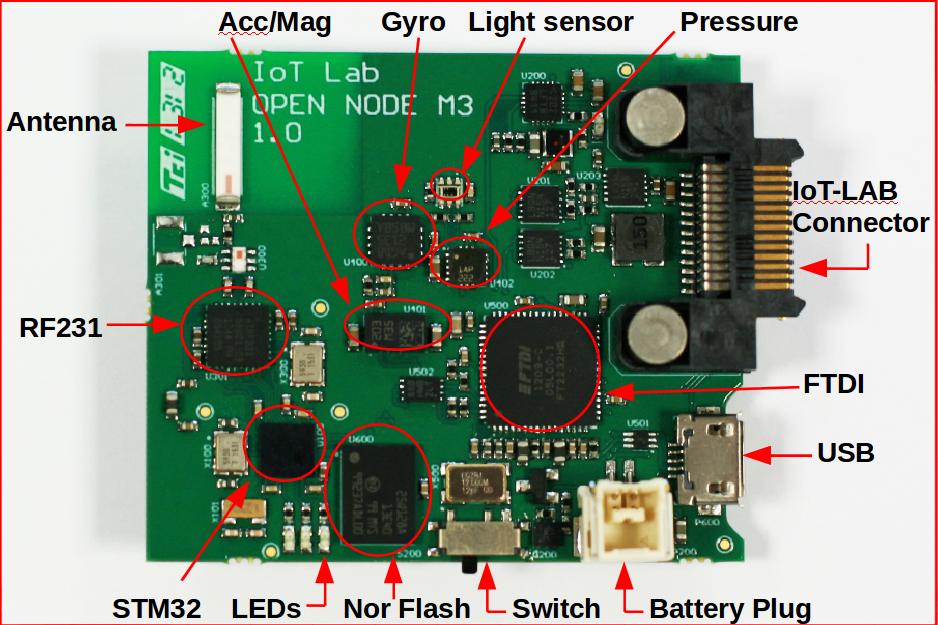
\includegraphics[width=90mm]{images/m3opennode.png}
\caption{Vue détaillée d'un nœud M3}
\end{figure}

Ces capteurs sont la source des données extérieures et la raison de déployer des CPS.

\subsection{Réseau de nœuds}

Les réseaux de capteurs ne sont généralement pas mis en réseau comme des ordinateurs classiques, où chaque nœud du réseau peut accéder directement à internet.

Ici le réseau est de type \emph{mesh}, c'est à dire qu'un nœud est connecté à internet, il est appelé le \emph{border router}, et que les autres sont ou reliés au \emph{border router} ou à un autre nœud indirectement connecté au \emph{border router}. Un exemple de ce type de réseau est montré en Figure \ref{mesh-network}.

\begin{figure}[ht!]
\centering
\label{mesh-network}
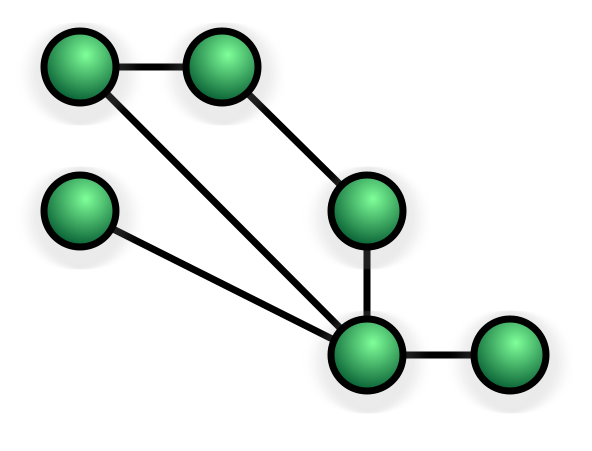
\includegraphics[scale=0.3]{images/mesh-network.png}
\caption{Topologie d'un réseau mesh, le border routeur peut potentiellement être n'importe lequel de ces nœuds}
\end{figure}

De cette manière pour récupérer du contenu sur internet un nœud peut avoir besoin d'effectuer plusieurs bonds. Également la connexion entre nœuds n'est pas filière mais par ondes radio, réduire au maximum les communications entre nœuds est donc un enjeu de gain de temps puisque les débits de communication sont très faible et de batterie puisque qu'une communication peut impacter tout un réseau dans certains structures.

\subsection{Principales différences}

De par ces différences le développement logiciel est radicalement différent de ce que l'on peut trouver lorsque l'on cible un ordinateur «classique».

Dans notre cas ces limites sont dues au langage de développement, le langage C, qui n'est pas compilé pour utiliser la \emph{libc} standard, non disponible sur l'environnement \emph{Contiki}. Cette restriction, entre autre, empêche l'utilisation de générateur de code.

Bien que possible sur un environnement \emph{Contiki} l'allocation dynamique de mémoire ne doit pas se faire en utilisant le classique \emph{malloc}. En effet ce dernier gère mal la fragmentation de la mémoire. Pour palier à cela \emph{Contiki} met à disposition des développeurs d'autres méthodes telles que \emph{memb} et \emph{mmem}.\footnote{https://github.com/contiki-os/contiki/wiki/Memory-allocation}

Pour rester proportionné à l'espace disque et à la puissance de calcul des nœuds \emph{Contiki} utilise en système de fichiers spécifique nommé \emph{Coffee} qui est une  implémentation du \emph{Contiki File System}\footnote{https://github.com/contiki-os/contiki/wiki/File-systems}, CFS. Ce dernier empêche l'utilisation des fonctions habituelles de gestion d'accès disque telle que \emph{fopen}.

\section{Testbed FIT IoT-lab}

FIT est un projet financé par divers organismes de l'enseignement supérieurs et de la recherche afin de mettre à disposition des entreprises et des chercheurs des structures pour les aider dans leurs travaux.

IoT-lab\footnote{https://www.iot-lab.info/} est une infrastructure permettant l'accès à différents sites en France hébergeant du matériel dédié à l'Internet des Objets.

FIT permet l'accès à plus de 2700 nœuds répartis sur 7 différents testbed tel qu'à Rennes, Grenoble ou Rocquencourt. Les testbeds proposent jusqu'à 3 architectures différentes, dont des \emph{m3}.

Voir annexe \ref{iot-lab} en page \pageref{iot-lab} pour la distribution détaillée des différents nœuds.

La réservation de nœuds se fait directement sur le site web. L'utilisateur a libre choix sur le site, le nombre et le type de nœud. Dans la limite des ressources disponibles et pour une durée conseillée d'au maximum 2 heures.

Une fois des nœuds réservés et obtenus il est possible d'y déployer un nouveau firmware. Toutes ces opérations, de la réservation de nœuds au flashage d'un nouveau firmware, sont directement réalisable en ligne de commande\footnote{https://www.iot-lab.info/tutorials/experiment-cli-client/}.

\section{model@runtime, Kevoree et KMF}

\subsection{model@runtime}

Le développement de réseaux distribués de machines de plus en plus complexes a amené la volonté et le besoin de pouvoir les reconfigurer plus aisément. L'intérêt peut être de mettre à jour un module fonctionnant sur une machine tout en minimisant le temps durant lequel le module ne sera pas fonctionnel.

Pour cela le paradigme du \emph{model@runtime} utilise un modèle servant à définir l'architecture détaillée d'un réseau à un instant \emph{t}.

Cette approche fonctionne sur des réseaux d'ordinateurs et de serveurs \cite{fouquet} et l'objectif de la thèse de \paco est de prouver que cette approche fonctionne également pour l'Internet des Objets.

\subsection{KMF}

\emph{KMF}, Kevoree Modeling Framework\footnote{http://kevoree.org/kmf/}, est un langage de modeling s'inspirant de \emph{EMF}, Eclipse Modeling Framework\footnote{http://www.eclipse.org/modeling/emf/}, mais conçut pour répondre aux besoins du \emph{model@runtime}.

L'objectif de \emph{KMF} est de, à partir d'un méta-modèle, produire une structure de données et des outils de manipulation.

\subsection{\label{kevoree}Kevoree}

\emph{Kevoree} est un projet open-source implémentant le paradigme du \emph{model@runtime}. Les versions principales sont écrites en \emph{Java} et en \emph{Javascript} mais des implémentations en \emph{C} et \emph{C++} ont également été implémentées. Chaque version de \emph{Kevoree} est basée sur une version de \emph{KMF}. 

\emph{Kevoree} offre des mécanismes de comparaison et de fusion de modèles pour permettre l'adaptation de systèmes distribués.

\subsubsection{Kevoree-c}

La version utilisée durant ce stage est \emph{kevoree-c}\footnote{https://github.com/kYc0o/kevoree-c-reloaded} réalisée par \paco dans le cadre de sa thèse. Contrairement aux autres versions de \emph{Kevoree} celle-ci n'a pas été obtenue par génération depuis un méta-modèle mais a été écrite à la main.


%les différentes versions
%Chargement de binaire, ELF loader1
%surtout faire la transition sur le besoin de produire une implémentation depuis un modèle de Kevoree écrit en KMF

    %\setcounter{section}{0}
\section{Premier développement sur Contiki}
Pour mieux appréhender la variété de l'environnement et des outils la première tâche qui m'a été confiée n'était pas au cœur de ses systèmes. J'ai tout d'abord lu l'article \citep{acostapadilla} pour me familiariser avec cet environnement. 

Les nœuds \emph{m3} étant uniquement capable d'exécuter du code déjà compilé il a fallu que je mette en place un environnement dit de \emph{Cross-compilation}, ou compilation croisée, qui consiste à produire un code binaire exécutable par une machine ayant une architecture différente de celle servant au développement.

Pour développer un nouveau module pour \emph{Contiki} il suffit d'en récupérer les sources\footnote{https://github.com/iot-lab/contiki}, de se placer dans le répertoire contenant les sources d'un module et de le compiler en précisant l'architecture cible, iotlab-m3.

\lstset{language=bash, captionpos=b, caption=Résumé des étapes de compilation}
\begin{lstlisting}[frame=single]
git clone https://github.com/iot-lab/contiki
cd contiki/example/hello-world
make TARGET=iotlab-m3
\end{lstlisting}

Cette compilation produira un firmware contenant \emph{Contiki}, le module courant ainsi que tout autre module marqué en dépendance. Ce firmware pourra directement être flashé sur un nœud \emph{m3}.

\section{Compression des modèles}

Pour pouvoir s'adapter et selon le principe du \emph{model@runtime} chaque nœud d'un réseau IoT doit comparer le nouveau modèle du réseau avec le courant et en déduire s'il doit se modifier. Il est donc nécessaire que le nouveau modèle soit échangé entre tous les nœuds. Dans un soucis de temps de développement et puisque cela n'impacte pas l'idée de \emph{model@runtime} l'implémentation de \emph{kevoree-c} ne compresse pas les modèles avant de les transmettre aux pairs voisins.

\subsection{État de l'art}

Puisque aucun algorithme de compression de données n'est fourni avec \emph{Contiki} j'ai d'abord commencé par en chercher implémentés en \emph{C}, recommandés pour les systèmes embarqués et disponibles en sources libres dans des licences permettant leurs réutilisations.

L'objectif étant d'avoir le meilleur taux de compression tout en restant le moins demandeur de ressources matérielles, en particulier en mémoire RAM.

Les implémentations retenues et étudiées sont \emph{Huffman}, \emph{fastlz}\footnote{http://fastlz.org/} et \emph{lzf} \footnote{http://oldhome.schmorp.de/marc/liblzf.html}.

Les résultats ont été obtenus en utilisant l'outil \emph{Massif}\footnote{http://valgrind.org/docs/manual/ms-manual.html} de la suite d'outils Valgrind. \emph{Massif} permet de mesurer l'utilisation de différentes zones mémoire lors de l'exécution d'un programme. Par défaut seul l'utilisation du tas est mesuré mais la pile peut également l'être après configuration. Les fichiers de données produits sont binaires mais peuvent être visualisés à l'aide de l'outil \emph{msprint} fourni avec \emph{Massif}.

Les mesures étant faites sur un ordinateur classique d'architecture 64bit et non sur l'environnement de production la compilation a été réalisée en 32bit pour réduire la taille des adresses de pointeur manipulées et ainsi avoir des résultats plus fiables. Tous les algorithmes ont été utilisés en compression et en décompression sur plusieurs modèles différents représentatifs de ceux utilisés lors des expériences.

Les scripts utilisés pour automatiser les mesures et produire les résultats suivants sont disponibles sur Github\footnote{https://github.com/AlexandreRio/embedded-compression-benchmark}.

\subsection{Résultats mesurés}

Le taux de compression $\frac{taille~finale}{taille~initiale}$ moyens de chaque algorithme est mesuré sur un ensemble de fichier 14 fichiers représentant 7 modèles différents. Chaque modèle est représenté par un fichier facilement lisible par l'Homme et par une représentation minimaliste, sans caractère de mise en forme superflu.
\[
\begin{array}{lc}
Algorithme & Taux~de~compression \\
LZF & 0.174 \\
Huffman & 0.604 \\
Fastlz-1 & 0.179 \\
Fastlz-2 & 0.171 \\
Table~association & 0.641
\end{array}
\]

L'annexe \ref{comp-tabde} détaille les tailles avant et après compression pour l'ensemble de ces fichiers.

\begin{figure}[ht!]
\centering
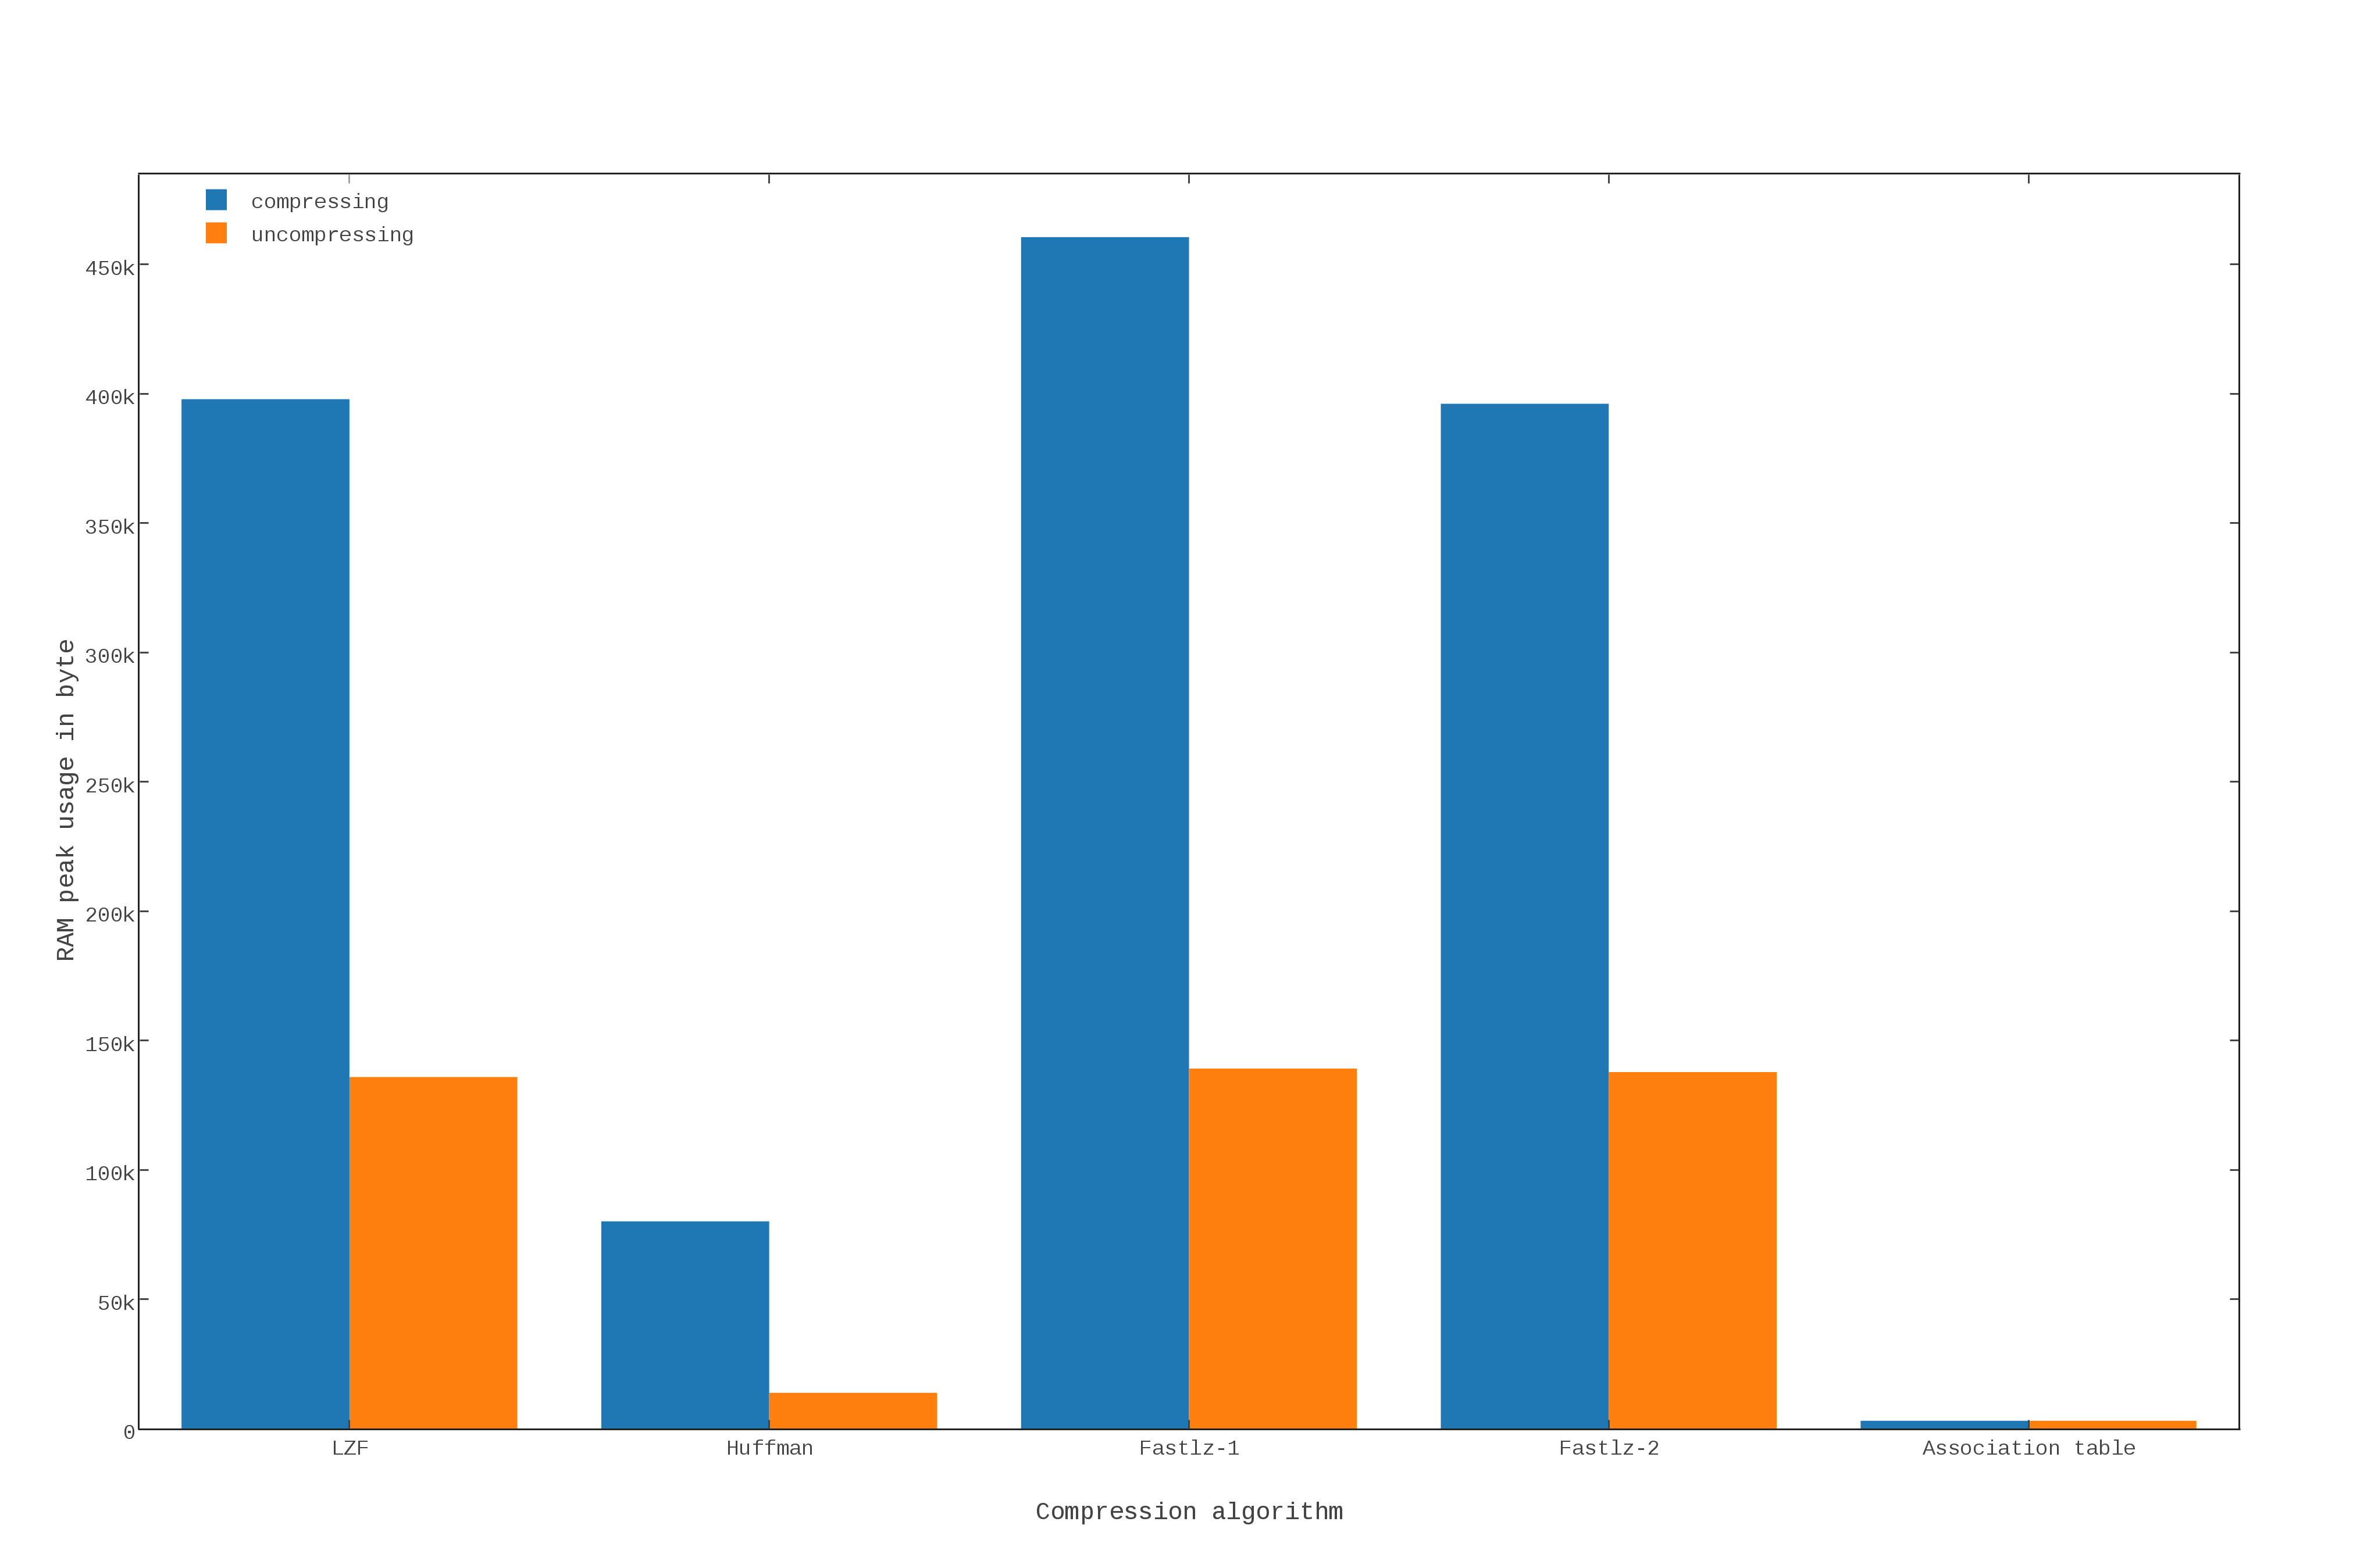
\includegraphics[scale=0.4]{images/comp-memory.png}
\caption{Pic moyen d'utilisation de la RAM en octet en fonction de l'algorithme de compression.}
\end{figure}

En réduisant la taille des buffers la taux de compression chute

\subsection{Table d'association}

Vue qu'aucune implémentation existante ne peut fonctionner sur \emph{Contiki} j'ai développé un programme de compression.

La structure générale et les mots-clés du fichier à compresser étant connus à l'avance la méthode la plus simple de compression est de réaliser une table d'association entre les mots les plus fréquemment utilisés et de les substituer par un code plus court.

Cette approche oblige tous les nœuds à connaître la table d'association utilisée pour compresser lors de la décompression. Cette table étant constante lors de la vie du programme elle peut être stockée en ROM, ce qui est important dans notre cas.

Pour obtenir cette table d'association j'ai réalisé un programme \emph{Java}, disponible sur Github\footnote{https://github.com/AlexandreRio/Contiki-compression-tools}, qui se base sur un ensemble de modèle. Le programme peut être paramétré pour produire une table plus au moins grosse, au détriment du taux de compression moyen.

Les premiers tests sur \emph{Contiki} ont d'abord consisté à simplement compressé une   chaine de caractères constante au programme, puis un fichier local au nœud et pour finir un fichier local au nœud envoyé à un second nœud qui le décompresse après réception. Le résultat attendu étant que le fichier obtenu après compression, transmission et décompression soit identique ou au moins sémantiquement identique.

Les expériences ont été réalisées sur le testbed FIT IoT-lab de Rocquencourt qui a l'avantage de ne compter que 24 nœuds M3 (voir annexe \ref{iot-lab}), ce qui est largement suffisant dans le cadre de cette expérience et permet d'être sur d'avoir des nœuds disponibles et de pouvoir les réserver pour plusieurs heures sans gêner d'autres expériences.

La transmission de données, ici de modèles, est particulière sur un réseau mesh et dans le cas de \emph{Kevoree}. Pour le \emph{model@runtime} la transmission de données est utilisée pour transmettre le nouveau modèle depuis $1$ nœud à $n-1$ nœuds, cette transmission a été appelée dissémination. Dans le cadre de mes expériences de test de compression avant transmission j'ai déployer plusieurs nœuds \emph{border router} possédant la nouvelle version du modèle et seulement $1$ possédant l'ancienne version. De cette manière et en prenant en compte comment l'algorithme de dissémination est implémentée le nœud possédant l'ancienne version pourra recevoir la nouvelle, découpées en morceaux, de tous les nœuds proches de lui et ainsi le recevoir plus vite et donc réduire le temps des expériences et par extension mon temps de développement.

Après avoir résolu les différents bugs liés à l'environnement, tel que le système de fichier, le code du programme de compression a déplacer afin de produire un module indépendant dans \emph{Contiki}. De ce fait n'importe quel autre module ou programme basé sur \emph{Contiki} peut utiliser cette fonction pour compresser ou décompresser des fichiers.

% vérifier les liens
Les sources de la version de compression seule \footnote{https://github.com/AlexandreRio/contiki/tree/usingOldKevoree/examples/compress} et de la compression et transmission \footnote{https://github.com/AlexandreRio/contiki/tree/usingOldKevoree/examples/compress-disseminate} sont disponibles sur Github.

\section{Parser spécifique}

\subsection{Tentatives de portage}

trop de limite,
\section{Compilation}

Le gros du stage pour le moment

\subsection{L'intérêt de générer du code}

\subsection{Un vrai compilateur et pas juste une transcription de modèle}
    \newtitle
    \section*{Conclusion}
\phantomsection
\addcontentsline{toc}{section}{Conclusion}

\subsection*{Avancement}
\phantomsection
\addcontentsline{toc}{subsection}{Avancement}
La réalisation d'un compilateur est une tâche longue et complexe, la génération de code implique une confiance dans le générateur, c'est pourquoi il doit être le plus lisible possible. Tant dans sa représentation intermédiaire que dans sa manière de générer du code.

À la rédaction de ce rapport, soit 3 semaines avant la fin du stage :
\begin{itemize}
\item le désérialiseur est partiellement implémenté, seul reste la gestion des liens \texttt{1-1} entre les classes,
\item l'intégration des outils de comparaison et d'adaptation développés pour \emph{Kevoree-C} reste à faire
\end{itemize}

Si \emph{kmfc} génère du code \emph{C} à partir d'un méta-modèle, certains cas sont ad-hoc au méta-modèle \emph{Kevoree}. Ces cas ont été documentés et expliqués directement dans le code source sous forme de commentaires.

\subsection*{Bilan}
\phantomsection
\addcontentsline{toc}{subsection}{Bilan}

Un compilateur fait le lien entre deux langages, dans le cadre de mon stage il s'agissait de lire des méta-modèles pour produire du code \emph{C} destiné à des systèmes embarqués. Bien que le code produit soit lui aussi destiné à être compilé il n'en reste pas moins de très bas niveau et demande de bonnes connaissances tant du langage en lui même que des systèmes exécutant le firmware produit.
Le passage d'un langage de haut niveau de modélisation à un langage très proche du matériel est une tâche très stimulante. À cela s'ajoute le fait de manipuler plusieurs langages de programmation, celui d'entrée du méta-modèle, celui dans lequel est implémenté le compilateur, \emph{Java}, celui du code généré, \emph{C}, sans oublier les différents outils venant se greffer au projet tels que le moteur de template \emph{Velocity} et \emph{cmake}.


\subsection*{Avenir}
\phantomsection
\addcontentsline{toc}{subsection}{Avenir}

La structure de \emph{kmf} permet de facilement ajouter en retirer des méthodes à générer. Il est donc possible de rapidement tester un nouveau firmware que l'on peut déployer directement sur le testbed.

En plus de pouvoir expérimenter des modifications sur le méta-modèle \emph{Kevoree} et obtenir immédiatement un le code \emph{C} correspondant \emph{kmfc} permet également d'expérimenter des représentations de données ou d'autres manières d'implémenter le \emph{model@runtime} en ne modifiant qu'une partie minime du code source.

%on peut envisager implémenter KMF 6? avec les times tree, biblio des 2 papiers, si possible

Dans l'optique d'optimisation il serait possible d'intégrer \emph{kmfc} à un autre outil afin de mesurer l'utilisation de la RAM en fonctionnement et la taille en ROM du firmware produit.
%    \newtitle
%    \section*{Résumé}
\addcontentsline{toc}{section}{Résumé}


%    \newtitle
%    \section*{Résumé}
\addcontentsline{toc}{section}{Abstract}


%    \newtitle
%\setlength{\baselineskip}{1.0\baselineskip}
%    \section*{Glossaire} % Pas de numérotation
\addcontentsline{toc}{section}{Glossaire}

\begin{itemize}
    \item \textbf{Abstraite (classe)} :  classe dont l'implémentation n'est pas complète et qui n'est pas instanciable. Elle sert de base à d'autres classes dérivées (héritées).

\end{itemize}

%    \newtitle
	\bibliographystyle{acm}
	\bibliography{references}
    \section*{Bibliographie} % Pas de numérotation
\addcontentsline{toc}{section}{Bibliographie}

\subsection*{Sites internet}

\begin{itemize}
    \item \emph{http://stackoverflow.com/} : stackoverflow
    \item \emph{http://www.wikipedia.org/} : Wikipedia
    \item \emph{http://docs.oracle.com/javase/6/docs/api/} : 
        Java™ Platform, Standard Edition 6
        API Specification
    % ML iot-lab
\end{itemize}

%    \newtitle
%    \listoffigures
%    \newtitle
    \section*{Annexes} % Pas de numérotation
\phantomsection
\addcontentsline{toc}{section}{Annexes}
\appendix
\renewcommand\thefigure{\thesection.\arabic{figure}}
\renewcommand\thelstlisting{\thesection.\arabic{lstlisting}}
\setcounter{figure}{0}
\setcounter{lstlisting}{0}
\setcounter{section}{1}
%\setcounter{subsection}{1}

\subsection{\label{iot-lab}Distribution des nœuds FIT iot-lab}


\begin{figure}[ht!]
\centering
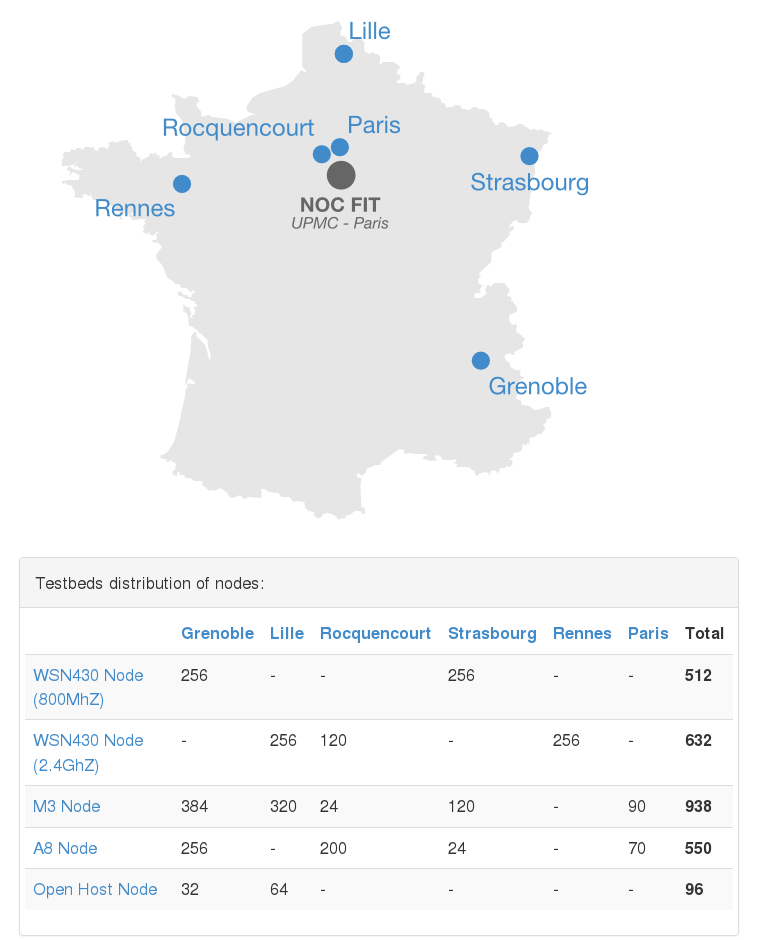
\includegraphics[scale=0.6]{images/iot-lab.png}
\caption{Source: https://www.iot-lab.info/deployment/}
\end{figure}

\subsection{\label{massif}Sortie de Massif}
\begin{figure}[ht!]
\centering
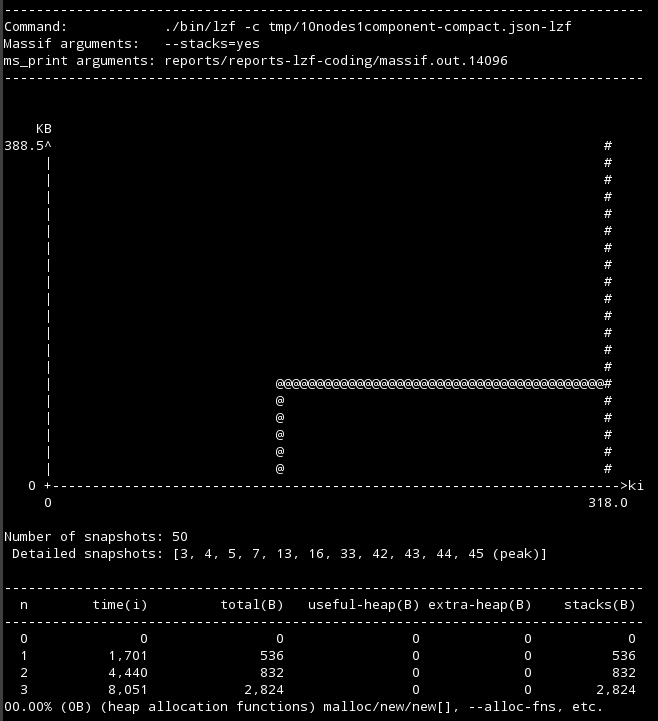
\includegraphics[scale=0.7]{images/msprint.png}
\caption{Exemple d'extrait de sortie de Massif, ici l'utilisation maximum de RAM est au snapshot 45 et est d'environ 400KB.}
\end{figure}

\begin{landscape}
\subsection{\label{comp-tabde}Compression de modèles}
\begin{figure}[ht!]
\centering
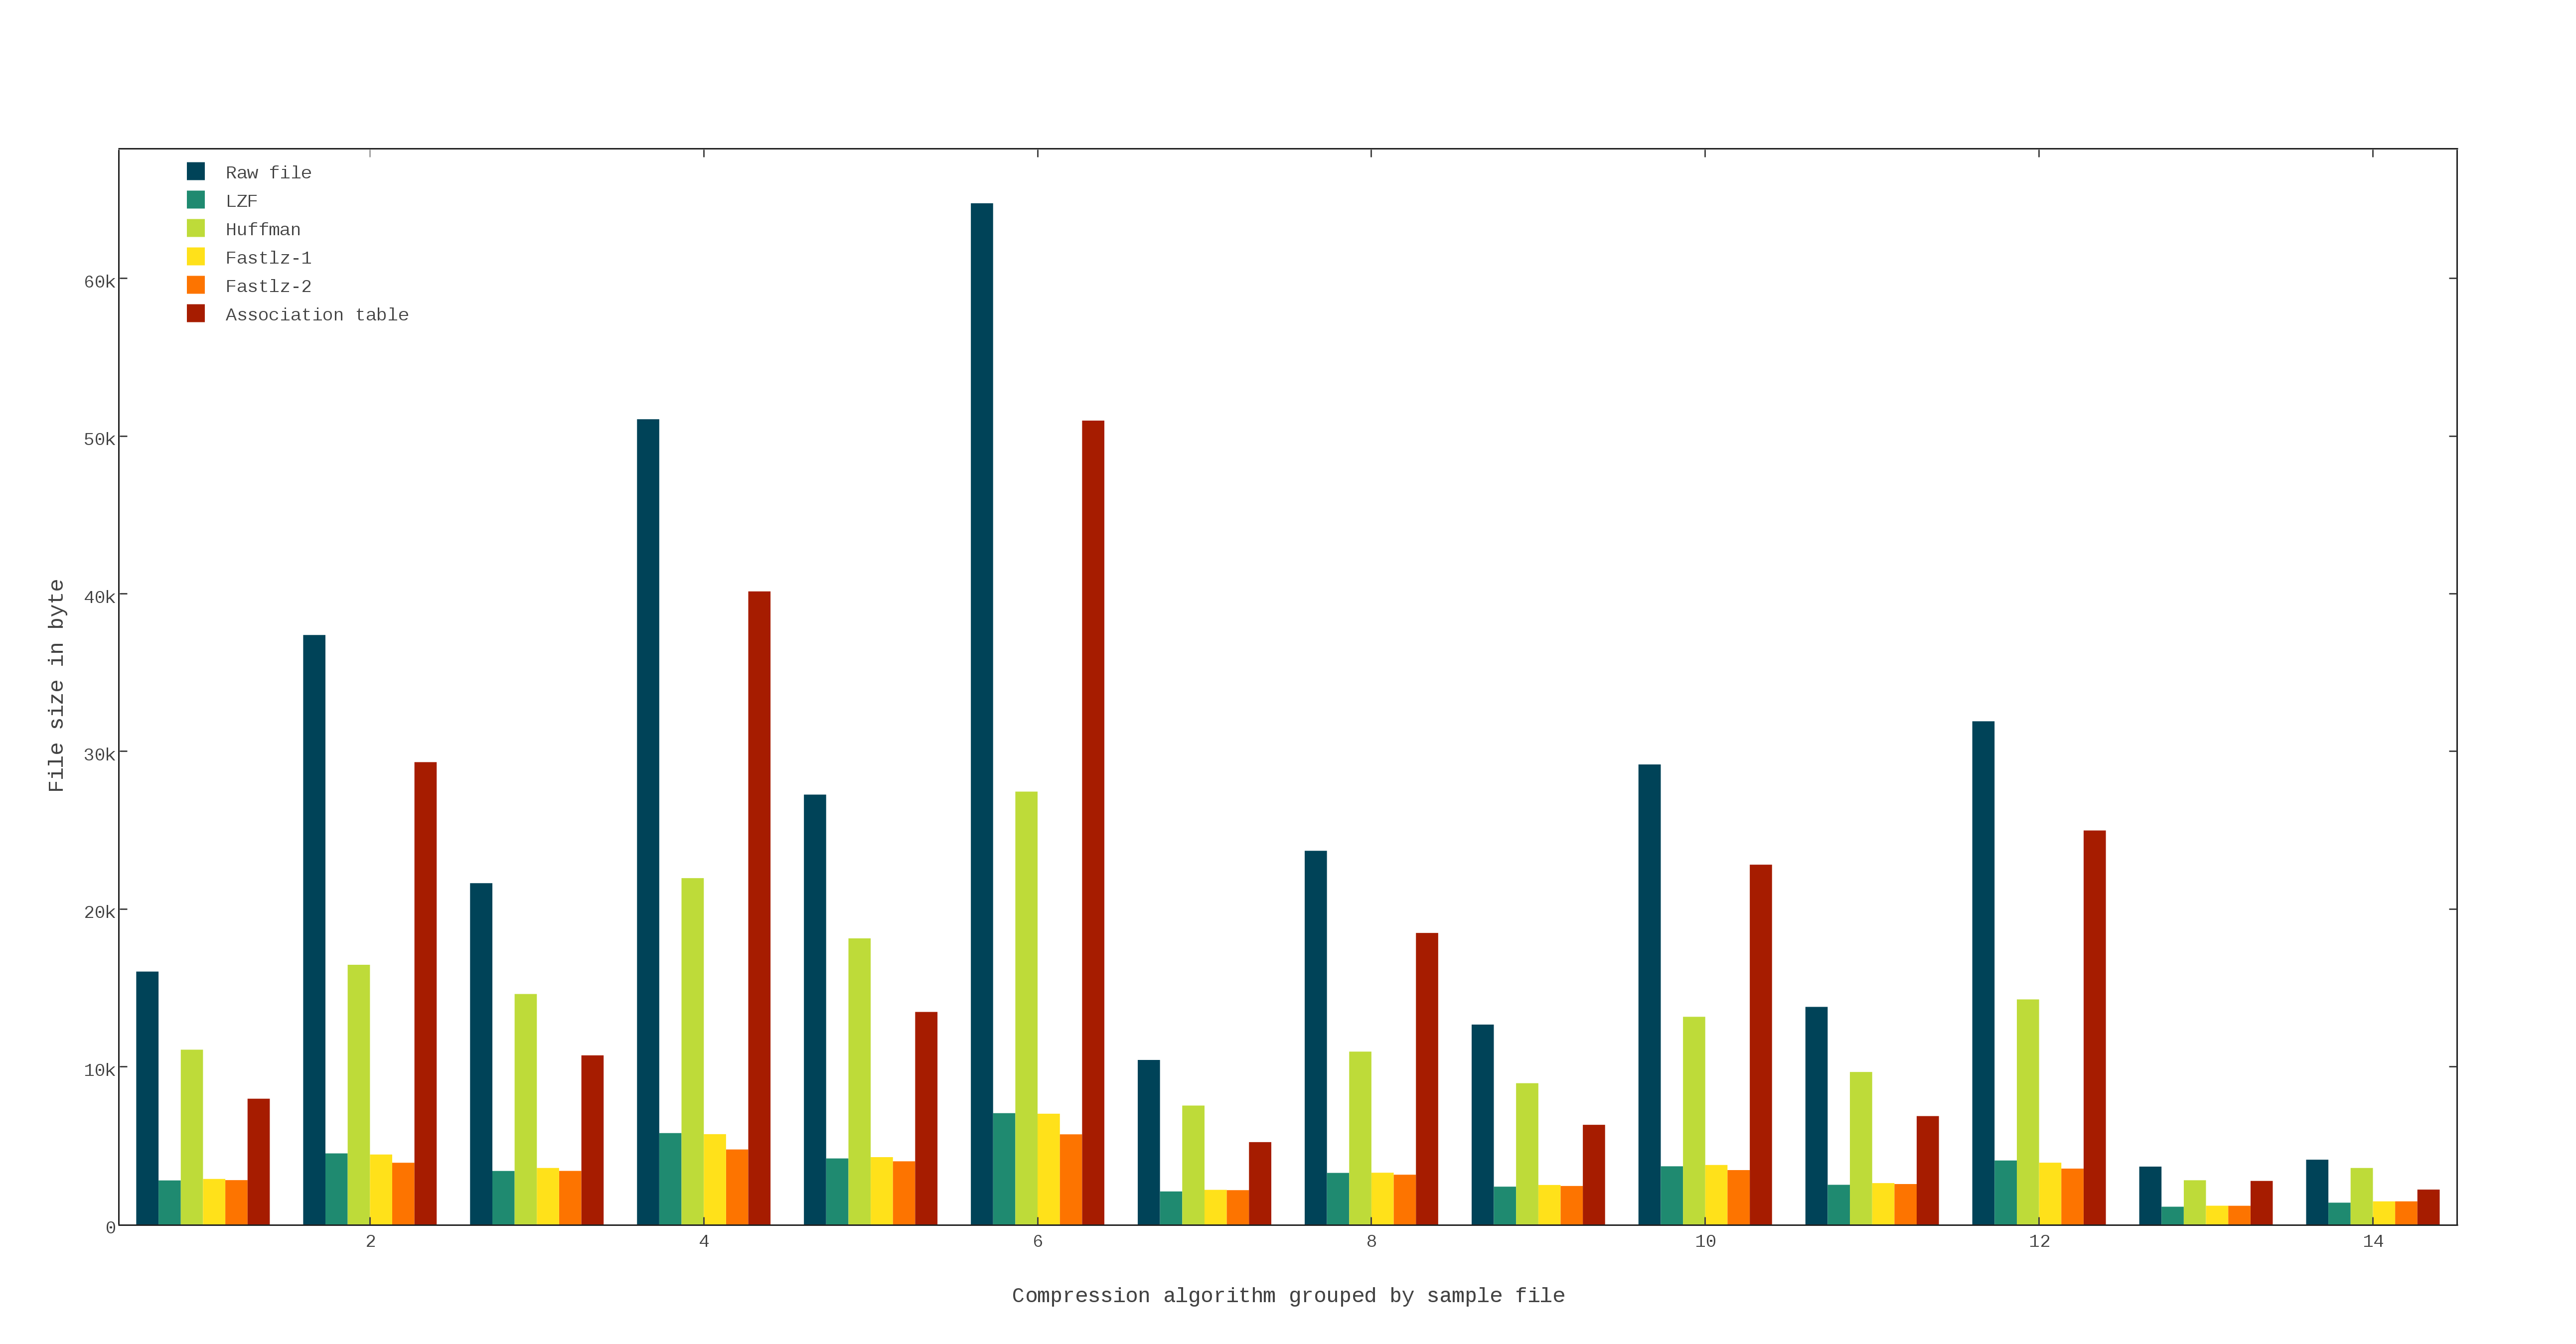
\includegraphics[scale=0.45]{images/compression.png}
\caption{Mesure de compression de modèles à l'aide de différents algorithmes}
\end{figure}
\end{landscape}

\begin{landscape}
\subsection{\label{kevoree-full-cd}Méta-modèle Kevoree}
\begin{figure}[ht!]
\centering
\fontsize{1mm}{4mm}\selectfont
\def\svgscale{0.28}
\input{images/kevoree-full-cd.pdf_tex}
\caption{Représentation du méta-modèle de Kevoree.}
\end{figure}
\end{landscape}

\lstset{
 language=C,
 captionpos=b,
 numbers=left,
 otherkeywords={},
 caption={Extrait du fichier Dictionary.h.}
}

\subsection{\label{dico-struct}Exemple de \texttt{struct} représentant une classe}
\begin{lstlisting}[frame=single]
typedef DictionaryValue* (*ftprDictionaryFindValuesByID)(Dictionary*, char*);
void initDictionary(Dictionary*);
Dictionary* new_Dictionary(void);

typedef struct _VT_Dictionary {
	VT_KMFContainer *super;
	/* KMFContainer */
	fptrKMFMetaClassName metaClassName;
	fptrKMFInternalGetKey internalGetKey;
	fptrKMFGetPath getPath;
	int (*fptrToJSON)(void*);
	fptrFindByPath findByPath;
	fptrDelete delete;
	/*Dictionary*/
	ftprDictionaryAddValues dictionaryAddValues;
	ftprDictionaryRemoveValues dictionaryRemoveValues;
	ftprDictionaryFindValuesByID dictionaryFindValuesByID;
} VT_Dictionary;

typedef struct _Dictionary {
	VT_Dictionary *VT;
	/* KMFContainer */
	KMFContainer *eContainer;
	/* Dictionary */
	char generated_KMF_ID[9];
	map_t values;
} Dictionary;
\end{lstlisting}
    \section*{Résumé}
\addcontentsline{toc}{section}{Abstract}


\end{document}
